\iflanguage{ngerman}
{\chapter{Ergebnisse}}
{\chapter{Results}}

\label{sec:results}

This chapter focuses on reviewing all of the work completed while utilizing all of the technologies to construct the application. Prior to integrating the technologies, each technique is evaluated independently.

\section{Smart Contract Performance }

Solidity-based smart contracts were created with the intention of integrating them into supply chains to maintain records of goods ownership and movement from one entity to another. It was vital to determine if the smart contracts were functioning properly or not shortly after developing them while keeping in mind the supply chain's sequence as shown in Figure \ref{Sequence Diagram}. 

\vspace{.5cm}

To verify this, we created several test cases and ran them using the Truffle tool. We kept in mind to verify the states, which are essentially the order of the supply chain, as well as store the ownership and movement of the product from one entity to another entity in each contract when doing the testing. The test cases are illustrated below utilizing a local network named "development," in which we are testing each contract by confirming the state of the product displayed in the Figure \ref{Data Model diagram}, as well as movement and ownership of the product using \ac{SKU}, \ac{UPC}, and owner ID and storing it into a buffer and then the cross checking them.

\vspace{.5cm}

\begin{lstlisting}[numbers=none, basicstyle=\ttfamily\tiny]
Using network 'development'.
Compiling your contracts...
===========================
> Everything is up to date, there is nothing to compile.
<----------------ACCOUNTS---------------->
Contract Owner: accounts[0]  0xad0BC114B5CF3F0797346fF1Fb1Daf1Cf5123395
Manufacturer: accounts[1]  0x4A9fe326Edc88F1f22940DC9F70BD391fB4218f8
Wholesaler: accounts[2]  0x5fB0Cd136C7A19E8E12F062548002B4460B0dC0d
Retailer: accounts[3]  0xc7D1C50D87B82E85b959DBC2cD9959bfc0480A5E
<-------TESTING CONTRACT FUNCTIONS------->
  Contract: SupplyChain
    Testing smart contract function produceItemByManufacturer() (14051ms)
    Testing smart contract function packageItemByManufacturer() (2723ms)
    Testing smart contract function sellItemByManufacturer() (2526ms)
    Testing smart contract function purchaseItemByWholesaler() (2037ms)
    Testing smart contract function shippedItemByManufacturer() (1566ms)
    Testing smart contract function receivedItemByWholesaler() (1542ms)
    Testing smart contract function sellItemByWholesaler() (1486ms)
    Testing smart contract function purchaseItemByRetailer() (2440ms)
    Testing smart contract function shippedItemByWholesaler() (1438ms)
    Testing smart contract function receivedItemByRetailer() (1380ms)
  10 passing (1m)
\end{lstlisting}

\vspace{.5cm}

According to the test scenarios, smart contracts are functioning well. Each contract will produce a transaction hash, which is simple to get and can be used to further verify information like as the date and time, amount of gas consumed, account used to deploy the contract, etcetera.

\subsubsection{Performance Over Test Networks}

Due to a built-in feature of the truffle tool that indicates how long it takes to build each contract as well as how long it takes to generate all of the contracts, we had to consider other options for our smart contracts. We tried to check the time taken by each network in order to get more knowledge, specifically taking into account the local network, Alfajores, and Rinkeby. We also considered testing out a different programming language to write our contracts in order to determine why Solidity is more effective than all of them.

\begin{figure}[h]
\centering
  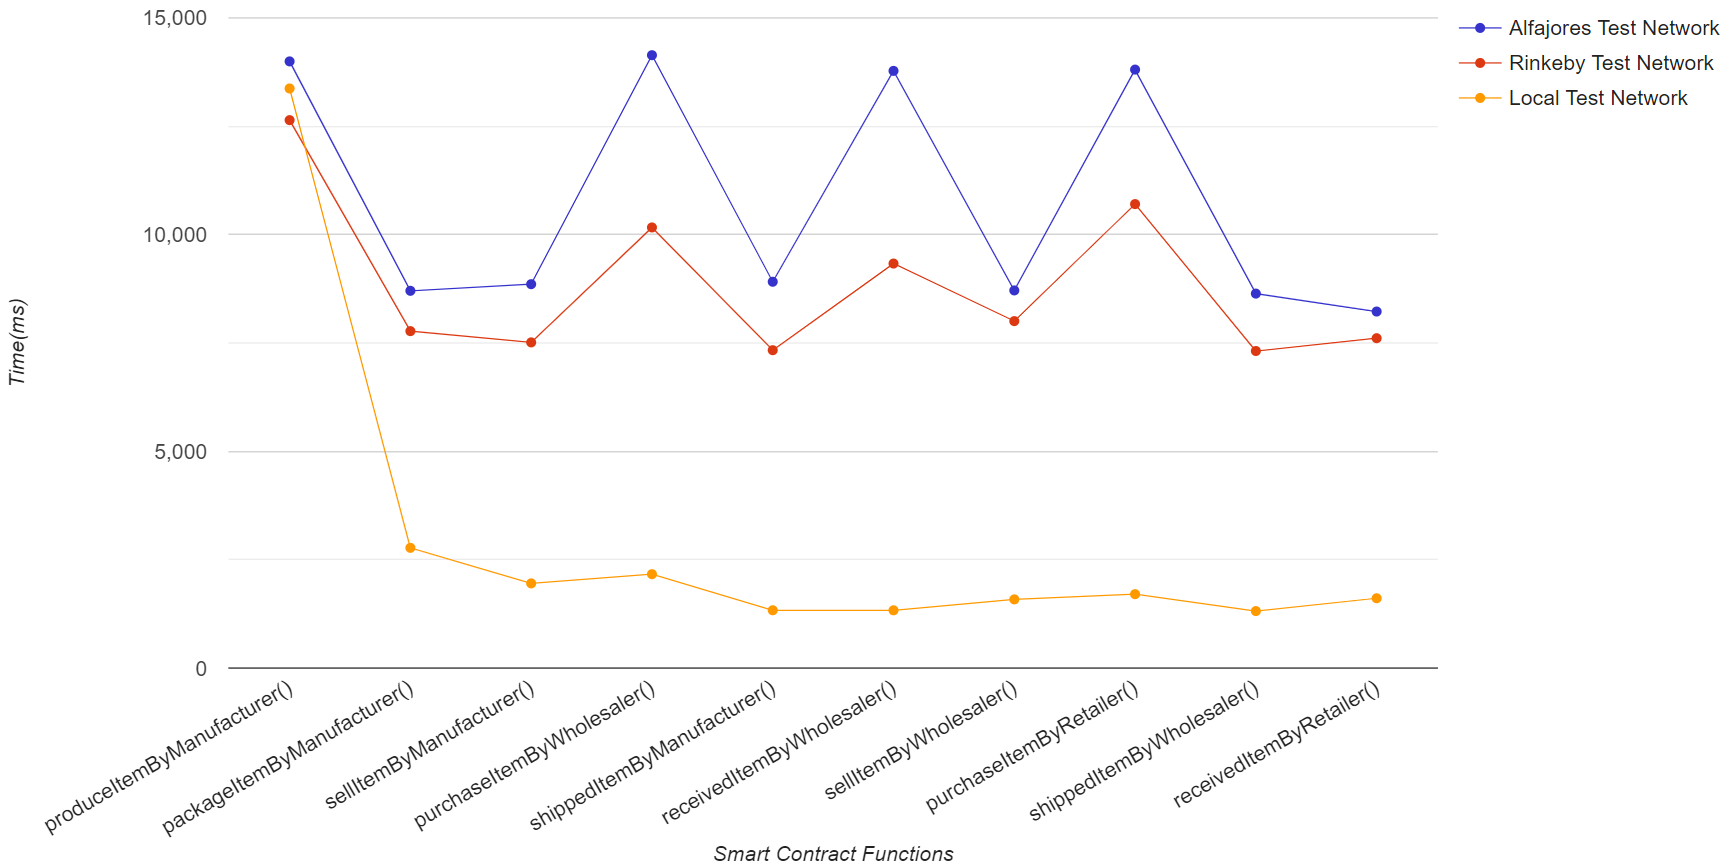
\includegraphics[width=15cm]{includes/figures/graph.png} 
  \caption{Performance across various networks}
  \label{Testing on networks}
\end{figure}

\vspace{.5cm}

It is obvious that the local network used far less time than the other two networks from Figure \ref{Testing on networks}. However, it was simpler to obtain CELO for Alfajores, the blockchain currency we used as gas for deployment and payment, than it was to acquire RinkebyETH for the Rinkeby test network. On the other hand, we can see that contract deployment was a little faster using the Rinkeby test network compared to the Alfajores test network.

\subsubsection{Contract Language Analogy}

We were decided from the outset to utilize Solidity to construct the smart contracts since it is a curly-bracket language meant to target the \ac{EVM}. C++, Python, and JavaScript have all had an impact on it. Solidity is statically typed and, among other things, enables inheritance, libraries, and sophisticated user-defined types. Furthermore, it receives frequent upgrades and breaking modifications, and new features are released on a regular basis. 

\vspace{.5cm}

JASON's and some issue with web3 libraries gave us the opportunity to explore more and to switch from Solidity to Vyper and learn more about the language. Because Vyper lacks \textit{Modifiers}, \textit{Class Inheritance}, \textit{Inline Assembly}, \textit{Function Overloading}, \textit{Operator Overloading}, and \textit{Binary Fixed Point}, a thorough examination of Vyper prompted us to chose Solidity once more. The usage of the following constructs might result in confusing or challenging to comprehend code, hence they are not included and to create final smart contracts, we continued to use Solidity as our primary language.

\section{\ac{MAS} Development}

We originally utilized JASON with a java-based interpreter to execute \ac{MAS}. To run \ac{MAS}, we downloaded the necessary scripts and libraries. Gradle and maven were then used for straightforward configuration and setting up the home variables. Then, in order to enable agent interaction, we created \texttt{mas2j} files after designing \texttt{asl} files for each agent. We introduced four agents: \texttt{supplyChainAgent}, \texttt{manufacturerAgent}, \texttt{wholesalerAgent}, and \texttt{retailerAgent}. The \texttt{supplyChainAgent} is the primary agent who will engage other agents to achieve their objectives. As their names imply, the other agents will perform their respective tasks in an adaptive supply chain. Running the agents in the \ac{MAS} environment produced the following results.

\vspace{.5cm}

\begin{lstlisting}[numbers=none, basicstyle=\ttfamily\tiny]

<---------------INTERACTION BETWEEN AGENTS---------------->
supplyChainAgent : Starting SupplyChain with SmartContracts
supplyChainAgent : Hi, I am the owner of Contract
supplyChainAgent : Creating RetailerAgent
retailerAgent    : Hi, I am here
retailerAgent    : Checking Warehouse, and order
retailerAgent    : Ordering to wholesalerAgent
supplyChainAgent : Creating WholesalerAgent
wholesalerAgent  : Hi, I am here
wholesalerAgent  : Checking Warehouse, and order
wholesalerAgent  : Ordering to manufacturerAgent
supplyChainAgent : Creating ManufacturerAgent
manufacturerAgent: Hi, I am here
manufacturerAgent: Checking Warehouse, and Manufacturing
manufacturerAgent: Manufacturing Product
manufacturerAgent: Packaging Product
manufacturerAgent: Selling product to wholesalerAgent
wholesalerAgent  : Purchasing product from manufacturerAgent
manufacturerAgent: Shipping product to wholesalerAgent
wholesalerAgent  : Received product from manufacturerAgent
wholesalerAgent  : Selling product to retailerAgent
retailerAgent    : Purchasing product from wholesalerAgent
wholesalerAgent  : Shipping product to retailerAgent
retailerAgent    : Received product from wholesalerAgent
retailerAgent    : NOW SELL TO CUSTOMER!!
supplyChainAgent : SUPPLYCHAIN COMPLETE
\end{lstlisting}

\vspace{.5cm}

Due to the limitations of Java-based interpreter with \texttt{web3} package, we immediately switched to \ac{ASTRA} and JASON with a Python-based interpreter. However, all of them produced the same outcome as described above, despite the fact that the scripting of agents and the \ac{MAS} environment differed.

\vspace{.5cm}

\ac{ASTRA} agents, unlike JASON, are not written in \texttt{asl} files, and it also does not require a \texttt{mas2j} file to make all of the agents interact with one another. In \ac{ASTRA}, all of the agents' primary and secondary goals may be expressed in a single \texttt{astra} file. Agents are written in Java-style syntax, which makes it easier for coders to comprehend and write in the format. The primary means of interaction between agents in \ac{ASTRA} is through the usage of an \ac{ACL}. \ac{ASTRA} allows for direct contact through \ac{FIPA} \ac{ACL}-based message forwarding.

\vspace{.5cm}

Although \ac{ASTRA} is simpler to grasp, it suffers from the same restriction as JASON with its Java-based interpreter in that it cannot leverage the \texttt{web3} package to infuse \ac{BCT} into the \ac{MAS}. As a result, we decided to use JASON with a Python-based interpreter. It is being used after installing the \texttt{agentspeak} package using \ac{pip}. It utilizes the same \texttt{asl} file, but instead of a \texttt{mas2j} file, it initiates the agents interaction with a python script. It is as simple to run as any other Python script and works flawlessly when smart contract functionalities are added to it as \texttt{actions} of agents.

\section{Infuse \ac{BCT} in \ac{MAS} }

Following the creation of contracts, we began looking for an appropriate \ac{AOP} language that is compatible with the \texttt{web3} library and can be used by agents in a \ac{MAS} to generate smart contracts. In the last chapter, we discussed every solution we considered. 

\subsubsection{Finale Outcome}

Our main objective was to find a way to incorporate \ac{BCT} into \ac{MAS} and create smart contracts using JASON \ac{BDI} agents. One of our ideas was successful, and the infuse was effective. We tested the code several times to make sure it was running correctly by looking at the \texttt{contract address} and \texttt{transaction hashes} from ganache as we were deploying using local network, and each try was successful, as can be seen in the output from one of the evaluations below.

\vspace{.5cm}

\begin{lstlisting}[numbers=none, basicstyle=\ttfamily\tiny]
<---------------------SMART CONTRACTS AND AGENTS----------------------->
Deployed Contract Address: 0xc9f78D73aCAf603Fe2319682316268A39Cc5CBB7
Owner Address: accounts[0] 0xad0BC114B5CF3F0797346fF1Fb1Daf1Cf5123395
Manufacturer Address: accounts[1] 0x4A9fe326Edc88F1f22940DC9F70BD391fB4218f8
Wholesaler Address: accounts[2] 0x5fB0Cd136C7A19E8E12F062548002B4460B0dC0d
Retailer Address: accounts[3] 0xc7D1C50D87B82E85b959DBC2cD9959bfc0480A5E
<---------------------INTERACTION BETWEEN AGENTS-------------------->
supplyChainAgent : Starting SupplyChain with SmartContracts
supplyChainAgent : Hi, I am the owner of Contract, with account: 0xad0BC114B5CF3F0797346fF1Fb1Daf1Cf5123395
supplyChainAgent : Creating RetailerAgent
retailerAgent    : Hi, I am here, with account: 0xc7D1C50D87B82E85b959DBC2cD9959bfc0480A5E
retailerAgent    : Checking Warehouse, and order
retailerAgent    : Ordering to wholesalerAgent
supplyChainAgent : Creating WholesalerAgent
wholesalerAgent  : Hi, I am here, with account: 0x5fB0Cd136C7A19E8E12F062548002B4460B0dC0d
wholesalerAgent  : Checking Warehouse, and order
wholesalerAgent  : Ordering to manufacturerAgent
supplyChainAgent : Creating ManufacturerAgent
manufacturerAgent: Hi, I am here, with account: 0x4A9fe326Edc88F1f22940DC9F70BD391fB4218f8
manufacturerAgent: Checking Warehouse, and Manufacturing
manufacturerAgent: Manufacturing Product
manufacturerAgent: Tx produceItemByManufacturer successful with hash: 0x653ff850d6fdee68554ded12d07c3c570c1a8a7d9aafe64b6b3fe54abe1b05f8
manufacturerAgent: Packaging Product
manufacturerAgent: Tx packageItemByManufacturer successful with hash: 0xaaefbe4aaf9c4533f7bc0c83323140151e33cc896695deeb4d9596123683f4f2
manufacturerAgent: Selling product to wholesalerAgent
manufacturerAgent: Tx sellItemByManufacturer successful with hash: 0xadd6ee6dfe24c84b04562f66509842c74d7d5c9c20fbe15883773e30632ce582
wholesalerAgent  : Purchasing product from manufacturerAgent
wholesalerAgent  : Tx purchaseItemByWholesaler successful with hash: 0x9dc089278a6f8491d891c77215136ece5d69c94a37081f35428d9e6184b6da70
manufacturerAgent: Shipping product to wholesalerAgent
manufacturerAgent: Tx shippedItemByManufacturer successful with hash: 0xa020ef5eaed13aa05cbda1f92cb331fa6f4c493164a22ff11a43073b1ab289e0
wholesalerAgent  : Received product from manufacturerAgent
wholesalerAgent  : Tx receivedItemByWholesaler successful with hash: 0x19b414d448c142dbba17468c42f05d2012089e067442913f4c45a9c5011e5d9f
wholesalerAgent  : Selling product to retailerAgent
wholesalerAgent  : Tx sellItemByWholesaler successful with hash: 0xd562b49a09473dc00304abbb2d3be55f451a27406197a011d750329c62ee3c19
retailerAgent    : Purchasing product from wholesalerAgent
retailerAgent    : Tx purchaseItemByRetailer successful with hash: 0xfd490f1fa472c42d33612392f42756115d340df8685b95bb0a85203917ea0ff6
wholesalerAgent  : Shipping product to retailerAgent
wholesalerAgent  : Tx shippedItemByWholesaler successful with hash: 0x4104a12dbb37f565fa07191135eb35c249591e6c5832c2ba703f9c8746ac1bf8
retailerAgent    : Received product from wholesalerAgent
retailerAgent    : Tx receivedItemByRetailer successful with hash: 0xf19d8bc9b0ddd26e010b7fb19a319ddb8d0d390cf673756bff3299d8d36d2873
retailerAgent    : NOW SELL TO CUSTOMER!!
supplyChainAgent :  TxHashes stored in BLOCKCHAIN
supplyChainAgent : SUPPLYCHAIN COMPLETE
\end{lstlisting}

\vspace{.5cm}

After a successful implementation, we remained adamant on running it in Java and used the \texttt{web3j} package to integrate \ac{BCT} into \ac{MAS}. We attempted to use JASON with Java by converting the Python code into a Java application. The creation of a Java application containing Python code was successful, but when the \texttt{.mas2j} file was executed, it was unable to import the package \texttt{org.python} , which is necessary to start the program.